\documentclass{beamer}
\usetheme{metropolis}
\usepackage{graphicx}
\usepackage{amsmath}
\usepackage{tcolorbox}
\title{Digital Signal Processing: COSC360}
\author{Jordan Hanson}
\institute{Whittier College Department of Physics and Astronomy}

\begin{document}
\maketitle

\begin{frame}{Unit 1.3 Outline}
Previous lectures covered:
\begin{itemize}
\item Complex numbers 2: The Fourier series and Fourier transform (continuous and discrete)
\item \textit{Time-permitting}: The Laplace transform (continuous and discrete)
\end{itemize}
This lecture will cover: (Reading: \textbf{Chapter 2})
\begin{itemize}
\item \alert{Statistics and probability: the normal distribution and other useful distributions}
\item \alert{Noise: digitization and sampling}
\item Noise: Spectral properties of noise, ADC and DAC
\end{itemize}
\end{frame}

\section{Statistics and Probability: The Normal Distribution}

\begin{frame}[fragile]{Statistics and Probability: The Normal Distribution}
The \textit{mean}, $\mu$, and \textit{standard deviation}, $\sigma$, of a data set $\lbrace x_i \rbrace$ are defined as
\begin{align}
\mu &= \frac{1}{N}\sum_{i=1}^N x_i \\
\sigma^2 &= \frac{1}{N-1}\sum_{i=1}^N\left(x_i-\mu\right)^2
\end{align}
Octave commands:
\begin{verbatim}
x = randn(100,1);
mean(x)
std(x)
\end{verbatim}
\end{frame}

\begin{frame}[fragile]{Statistics and Probability: The Normal Distribution}
One nice theorem: \textit{The variance is the average of the squares minus the square of the average.}  Let $\langle x \rangle$ represent the average of the quantity or expression $x$.  We have
\begin{equation}
\sigma_x^2 = \langle x^2 \rangle - \langle x \rangle^2
\end{equation}
Proof: observe on board.
\end{frame}

\begin{frame}[fragile]{Statistics and Probability: The Normal Distribution}
\small
\textbf{Note}: There is a distinction between the \textit{process or signal process} and the \textit{the data}.  Just because the data has a given $\mu$ and $\sigma$ does not imply that the signal process has or will continue to have the exact same values of $\mu$ and $\sigma$.  The underlying process could be \textit{non-stationary}.
\begin{figure}
\centering
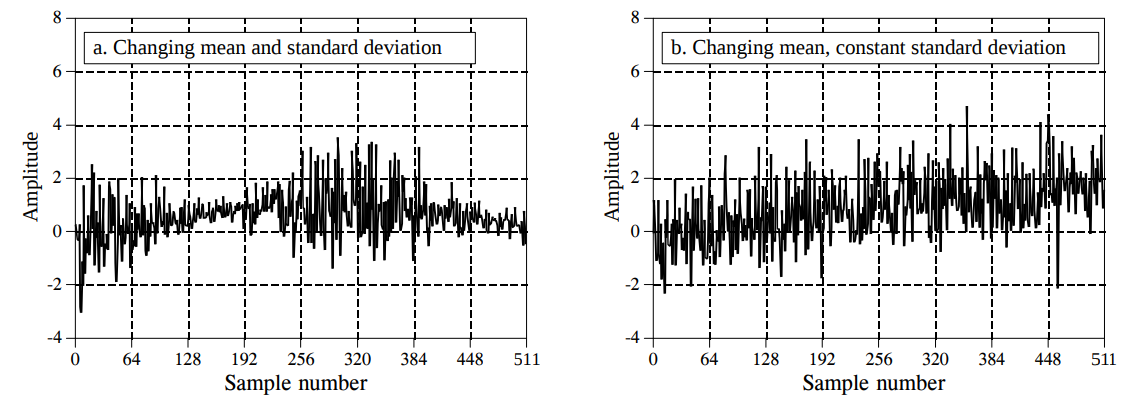
\includegraphics[width=0.9\textwidth]{figures/non_stationary.png}
\caption{\label{fig:non_stationary} Signal processes in (a) and (b) are considered \alert{non-stationary} because one or both of $\mu$ and $\sigma$ depend on time.}
\end{figure}
\end{frame}

\begin{frame}[fragile]{Statistics and Probability: The Normal Distribution}
\small
\textbf{A histogram} is an object that represents the frequency\footnote{Careful: the word frequency refers to the number of occurences in the data, not a sinusoidal frequency.} of particular values in a signal.  For example, below is a histogram of 256,000 numbers drawn from a probability distribution:
\begin{figure}
\centering
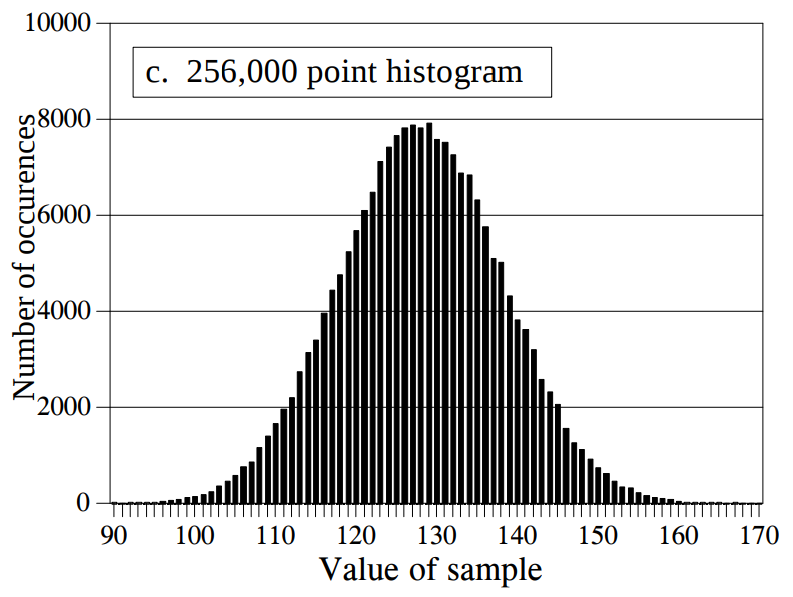
\includegraphics[width=0.45\textwidth]{figures/hist.png}
\caption{\label{fig:hist} The histogram contains counts versus sample values.}
\end{figure}
\end{frame}

\begin{frame}[fragile]{Statistics and Probability: The Normal Distribution}
The following octave code should reproduce something like Fig. \ref{fig:hist} from the textbook:
\begin{verbatim}
x = randn(256000,1)*10.0+130.0;
[b,a] = hist(x,100);
plot(a,b,'o');
\end{verbatim}
The function \textit{randn(N,M)} draws $N \times M$ numbers from a normal distribution and returns them in the size the user desires.  The function \textit{hist(x,N)} creates $N$ bins and sorts the data $x_i$ into them.
\end{frame}

\begin{frame}[fragile]{Statistics and Probability: The Normal Distribution}
\small
For data that is appropriately stationary, we can use histograms to estimate $\mu$ and $\sigma$ faster, since we only have to loop over bins rather than every data sample.  Let $H_i$ represent the counts in a given bin, and $i$ represent the bin sample.  We have:
\begin{align}
\mu &= \frac{1}{N}\sum_{i=1}^{M}i H_i \label{eq:histmean} \\
\sigma^{2} &= \frac{1}{N-1}\sum_{i=1}^M \left(i-\mu\right)^2 H_i \label{eq:histvar}
\end{align}
To obtain the mean in signal \textit{amplitude}, you'll have to convert bin number to amplitude.
\end{frame}

\begin{frame}[fragile]{Statistics and Probability: The Normal Distribution}
\small
\begin{table}
\begin{tabular}{c}
3.1 \\
-0.03 \\
1.2 \\
0.2 \\
-0.7 \\
-1.45 \\
2.2 \\
-0.05 \\
0.93 \\
0.21 
\end{tabular}
\caption{\label{tab:hist} Using Eq. \ref{eq:histmean} and \ref{eq:histvar}, find estimates of $\mu$ and $\sigma$ for this data.}
\end{table}
\begin{verbatim}
x = [...];
[b,a] = hist(x,4); %(How many bins?)
\end{verbatim}
\end{frame}

\begin{frame}[fragile]{Statistics and Probability: The Normal Distribution}
\small
Some vocabulary:
\begin{itemize}
\item \textbf{normalization} - Total probability is 1.0.  For pdf - the integral from $[-\infty,\infty]$ is 1.0.  For pmf - the sum from $[-\infty,\infty]$ is 1.0.
\item \textbf{pmf} - Probability mass function: A \textit{normalized continuous function} that gives the probability of a value, given the value.
\item \textbf{histogram} - Histograms are an attempted measurement of the pmf by breaking the data into discrete bins.  Histograms can be \textit{normalized} as well.
\item \textbf{pdf} - Probability density function: A \textit{normalized continuous function} that gives the probability density of a value, given the value.  Integrating the \textit{normalized} pdf between two values gives the probability of observing data between the given values.
\end{itemize}
\end{frame}

\begin{frame}[fragile]{Statistics and Probability: The Normal Distribution}
\begin{figure}
\centering
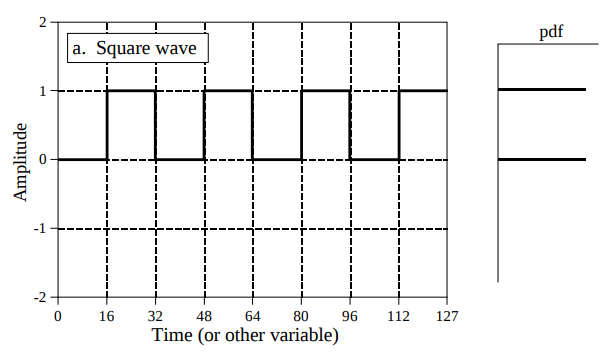
\includegraphics[width=0.7\textwidth]{figures/squarepdf.png}
\caption{\label{fig:squarepdf} The square-wave signal spends equal time at 0.0 and 1.0, and the probability density function reflects that.}
\end{figure}
\end{frame}

\begin{frame}[fragile]{Statistics and Probability: The Normal Distribution}
\begin{figure}
\centering
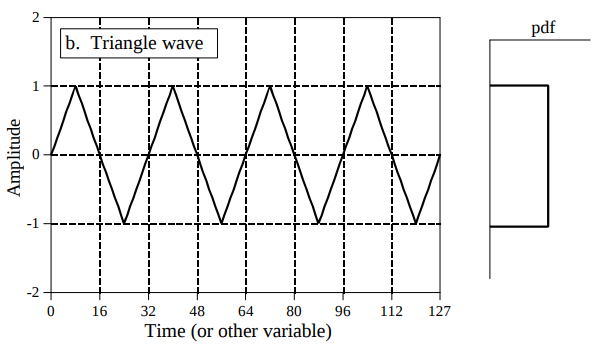
\includegraphics[width=0.7\textwidth]{figures/trianglepdf.png}
\caption{\label{fig:trianglepdf} The triangle-wave signal spends equal time at all values \textit{between} 0.0 and 1.0, and the probability density function reflects that.}
\end{figure}
\end{frame}

\begin{frame}[fragile]{Statistics and Probability: The Normal Distribution}
\begin{figure}
\centering
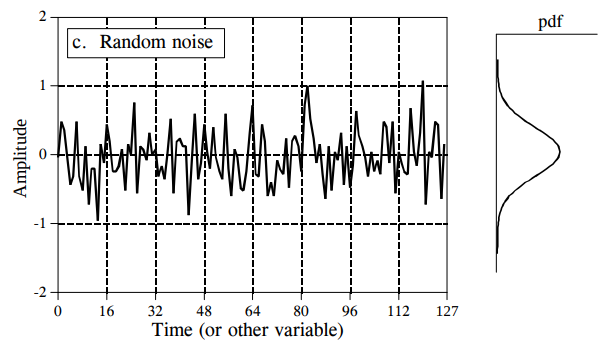
\includegraphics[width=0.7\textwidth]{figures/randnpdf.png}
\caption{\label{fig:randnpdf} The random noise \textit{usually} spends time near 0.0, but rarely it fluctuates to larger values.}
\end{figure}
\end{frame}

\begin{frame}{Normal distribution}
\textbf{Normally distributed} data decreases in probability at a rate that is proportional (1) to the \textit{distance from the mean}, and that is proportional (2) to the \textit{probability itself.}
\begin{figure}
\centering
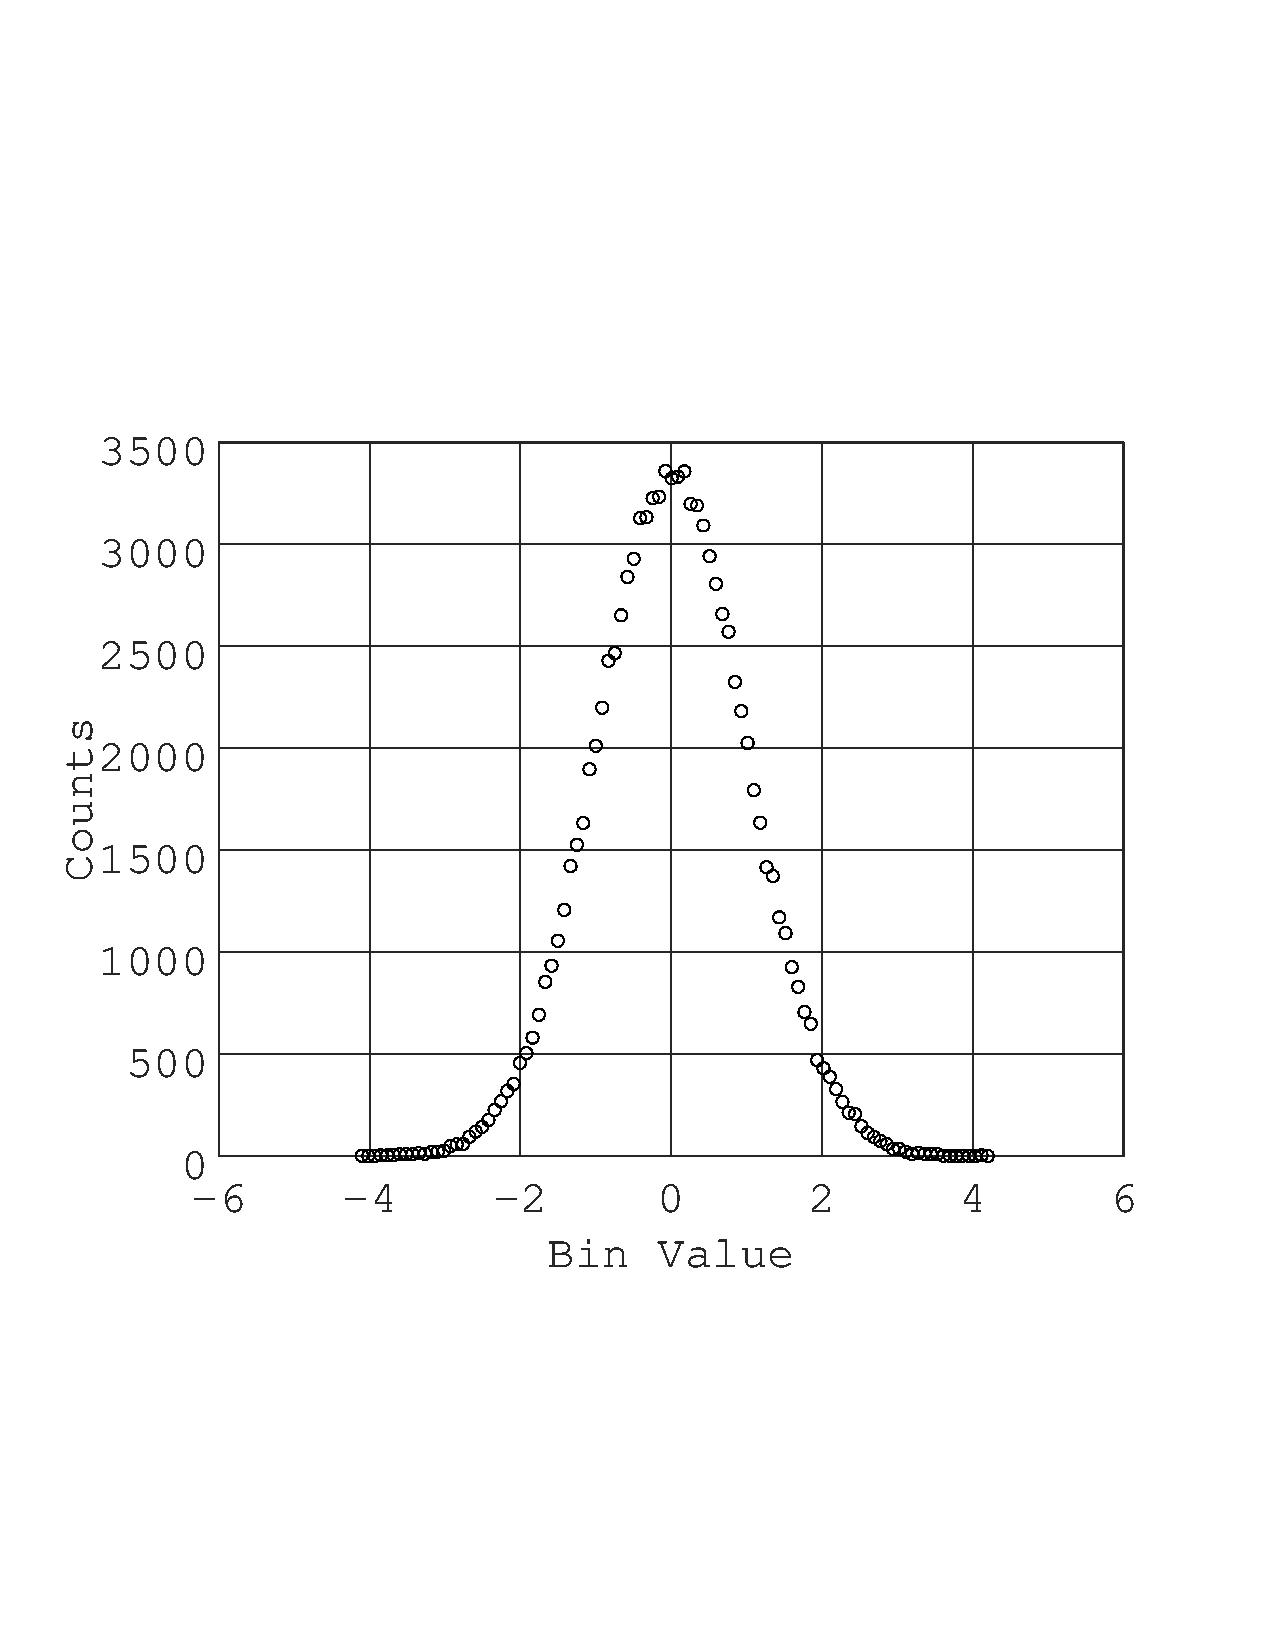
\includegraphics[width=0.5\textwidth,trim=0cm 6cm 0cm 6cm,clip=true]{figures/hist_binCount.pdf}
\caption{\label{fig:hist1} Normally distributed data counts decrease as measured further from the mean for \textit{two reasons.}}
\end{figure}
\end{frame}

\begin{frame}{Normal distribution}
\begin{tcolorbox}[colback=white,colframe=red!40!blue,title=Normal Distribution PDF]
\alert{Let $p(x)$ be the PDF of normally distributed data $x$ with mean $\mu$. In order to obey conditions (1) and (2), the function $p(x)$ must be described by the following differential equation, where $k$ is some constant.}
\alert{\begin{equation}
\frac{dp}{dx} = -k(x-\mu)p(x) \label{eq:normDiffeq}
\end{equation}}
\end{tcolorbox}
\end{frame}

\begin{frame}{Normal distribution}
Rearranging Eq. \ref{eq:normDiffeq}, we have
\begin{equation}
\frac{dp}{p} = -k(x-\mu) dx
\end{equation}
Integrating both sides gives
\begin{equation}
\ln(p) = -\frac{1}{2}k(x-\mu)^2+C_0
\end{equation}
Exponentiating,
\begin{equation}
p(x) = C_1 \exp\left(-\frac{1}{2}k(x-\mu)^2\right) \label{eq:normDiffeq2}
\end{equation}
Ensuring that the PDF is \textit{normalized} requires
\begin{equation}
\int_{-\infty}^{\infty} p(x) dx = 1
\end{equation}
\end{frame}

\begin{frame}{Normal distribution}
But how do we integrate Eq. \ref{eq:normDiffeq2}?  First, a change of variables.  Let $s = \sqrt{k/2}(x-\mu)$, so $ds = \sqrt{k/2}dx$.  Then, we have
\begin{equation}
C_1 \sqrt{\frac{2}{k}} \int_{-\infty}^{\infty} \exp(-s^2) ds = 1
\end{equation}
Squaring both sides, we have
\begin{equation}
C_1^2 \frac{2}{k} \left(\int_{-\infty}^{\infty} \exp(-s^2) ds\right)^2 = 1
\end{equation}
\end{frame}

\begin{frame}{Normal distribution}
Let's pretend the two factors of the integral involve different variables:
\begin{equation}
C_1^2 \frac{2}{k} \left(\int_{-\infty}^{\infty} \exp(-x^2) dx\right)\left(\int_{-\infty}^{\infty} \exp(-y^2) dy\right) = 1
\end{equation}
Now we have
\begin{equation}
C_1^2 \frac{2}{k} \int_{-\infty}^{\infty} \exp(-(x^2+y^2)) dx dy = 1
\end{equation}
Change to polar coordinates ($x^2 + y^2 = r^2$)
\begin{equation}
C_1^2 \frac{2}{k} \int_{0}^{\infty} \int_0^{2\pi} r\exp(-r^2) dr d\phi = 1
\end{equation}
\end{frame}

\begin{frame}{Normal distribution}
One more substitution: $u = r^2$, and $du = 2rdr$:
\begin{equation}
-\frac{C_1^2}{k} \int_0^{\infty}\int_0^{2\pi} \exp(-u) du d\phi = 1
\end{equation}
Solving for $C_1$, we find
\begin{equation}
C_1 = \sqrt{\frac{k}{2\pi}}
\end{equation}
Thus the pdf of normally distributed data is
\begin{equation}
p(x) = \sqrt{\frac{k}{2\pi}} \exp\left(-\frac{1}{2}k(x-\mu)^2\right)
\end{equation}
Let's defined $k = \frac{1}{\sigma_x^2}$ so that it's clear the exponent has the proper ratio of units:
\begin{equation}
\boxed{
p(x) = \sqrt{\frac{1}{2\pi\sigma_x^2}} \exp\left(-\frac{1}{2}\left(\frac{x-\mu}{\sigma_s}\right)^2\right)}
\end{equation}
\end{frame}

\section{Statistics and Probability: Programming with Octave}

\begin{frame}[fragile]{Statistics and Probability: Programming with Octave}
More on the \textit{hist} function in octave\footnote{I hope this works, but if not, it's ok.}
\begin{verbatim}
pkg install -forge io
pkg install -forge statistics
pkg load statistics
pkg help histfit
histfit(randn(1000,1))
histfit(rand(1000,1))
\end{verbatim}
Let's work out the $\sigma$ of a \textit{flat} distribution between $[0,1]$.  What is it for a flat distribution between $[-1,1]$?  (We can derive this by hand as well if we cannot access statistics package).
\end{frame}

\begin{frame}[fragile]{Statistics and Probability: Programming with Octave}
Some interesting notation for normal distributions:
\begin{equation}
N(\mu,\sigma) = \sqrt{\frac{1}{2\pi\sigma^2}} \exp\left(-\frac{1}{2}\left(\frac{x-\mu}{\sigma}\right)^2\right)
\end{equation}
Let's write a function \textbf{NGaus.m} that produces the Gaussian probability given $\mu$ and $\sigma$:
\begin{verbatim}
function ret = NGaus(mu,sigma,x)
    ...
endfunction
\end{verbatim}
\end{frame}

\begin{frame}[fragile]{Statistics and Probability: Programming with Octave}
Now let's write a function $NRand$ that sums $N$ uniformly-distributed (flat) random variables $x$:
\begin{verbatim}
function ret = NRand(n)
    ret = sum(rand(n,1));
endfunction
\end{verbatim}
Create a histogram of a few hundred outputs of $NRand$.  What do you notice about the pmf?  Let's plot $NGaus$ on the same axes as the histogram of $NRand$.  How do they compare? \\ \vspace{0.5cm}
We are on our way to producing $N(0,1)$ distributed numbers, and therefore our first \textbf{\alert{noise}} signals...
\end{frame}

\begin{frame}[fragile]{Statistics and Probability: Programming with Octave}
\small
The Box-Muller method for $N(0,1)$ distruted numbers:
\begin{align}
X_1 &= \sqrt{-2\ln(U)}\cos(2\pi V) \\
X_2 &= \sqrt{-2\ln(U)}\sin(2\pi V)
\end{align}
\textbf{Try this in octave...}
More vocabulary:
\begin{itemize}
\item \textbf{cdf} - Cumulative distribution function: Probability that a continuous random variable $X$ is less than some value $x$.  For a given pdf, the cdf $\Phi(X)$ is the integral of the total probability on $[-\infty,x]$.  The derivative of the pdf is related to the pdf via the fundamental theorem of calculus.
\end{itemize}
If the pdf follows $f(x)$, then 
\begin{equation}
\Phi(X\leq x) = \int_{-\infty}^{x} f(x) dx
\end{equation}
\end{frame}

\begin{frame}[fragile]{Statistics and Probability: Programming with Octave}
The cdf of $N(0,1)$ has an expected shape, but can't be expressed with elementary functions.
\begin{figure}
\centering
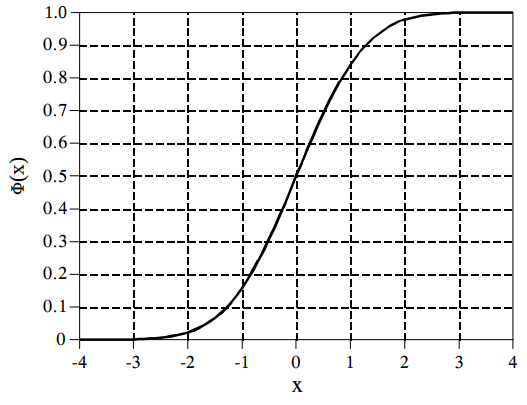
\includegraphics[width=0.5\textwidth]{figures/cdfgaus.png}
\caption{\label{fig:cdfgaus} The cumulative distribution of the normal distribution.  Although we can plot it, it's hard to write.  We will discuss the $erf$ and $erfc$ functions in the near future.}
\end{figure}
\end{frame}

\section{Statistics and Probability: Other Useful Distributions}

\begin{frame}[fragile]{Statistics and Probability: Other Useful Distributions}
\small
We now know how to obtain random uniform numbers (\textbf{rand}) in octave, and have algorithms (Box-Muller) and functions (\textbf{randn}) in octave for $N(0,1)$\footnote{This can be scaled to any $\mu$ and $\sigma$ values we need.}.  What if we require a \textit{different pdf}?  One technique is to use \textit{inverse transform sampling:}
\begin{enumerate}
\item For the pdf $p(x)$, work out the cdf $\Phi(x)$.
\item Generate a sample of uniform random numbers $u_i \in [0,1]$.
\item Call $\Phi^{-1}(u_i)$, that is, invert the cdf and plug in the list $u_i$ to the dependent variable.
\end{enumerate}
\textbf{Write an octave script that generates exponentially-distributed numbers, e.g. pdf $\propto \exp(-x)$.}
\end{frame}

\begin{frame}[fragile]{Statistics and Probability: Other Useful Distributions}
\small
\textbf{Octave Programming}: The scripts \textbf{meanStdDev...m} on Moodle demonstrate different digitized signals.  Examine the effect of changing the pdf of the noise from Gaussian to exponential.
\begin{figure}
\centering
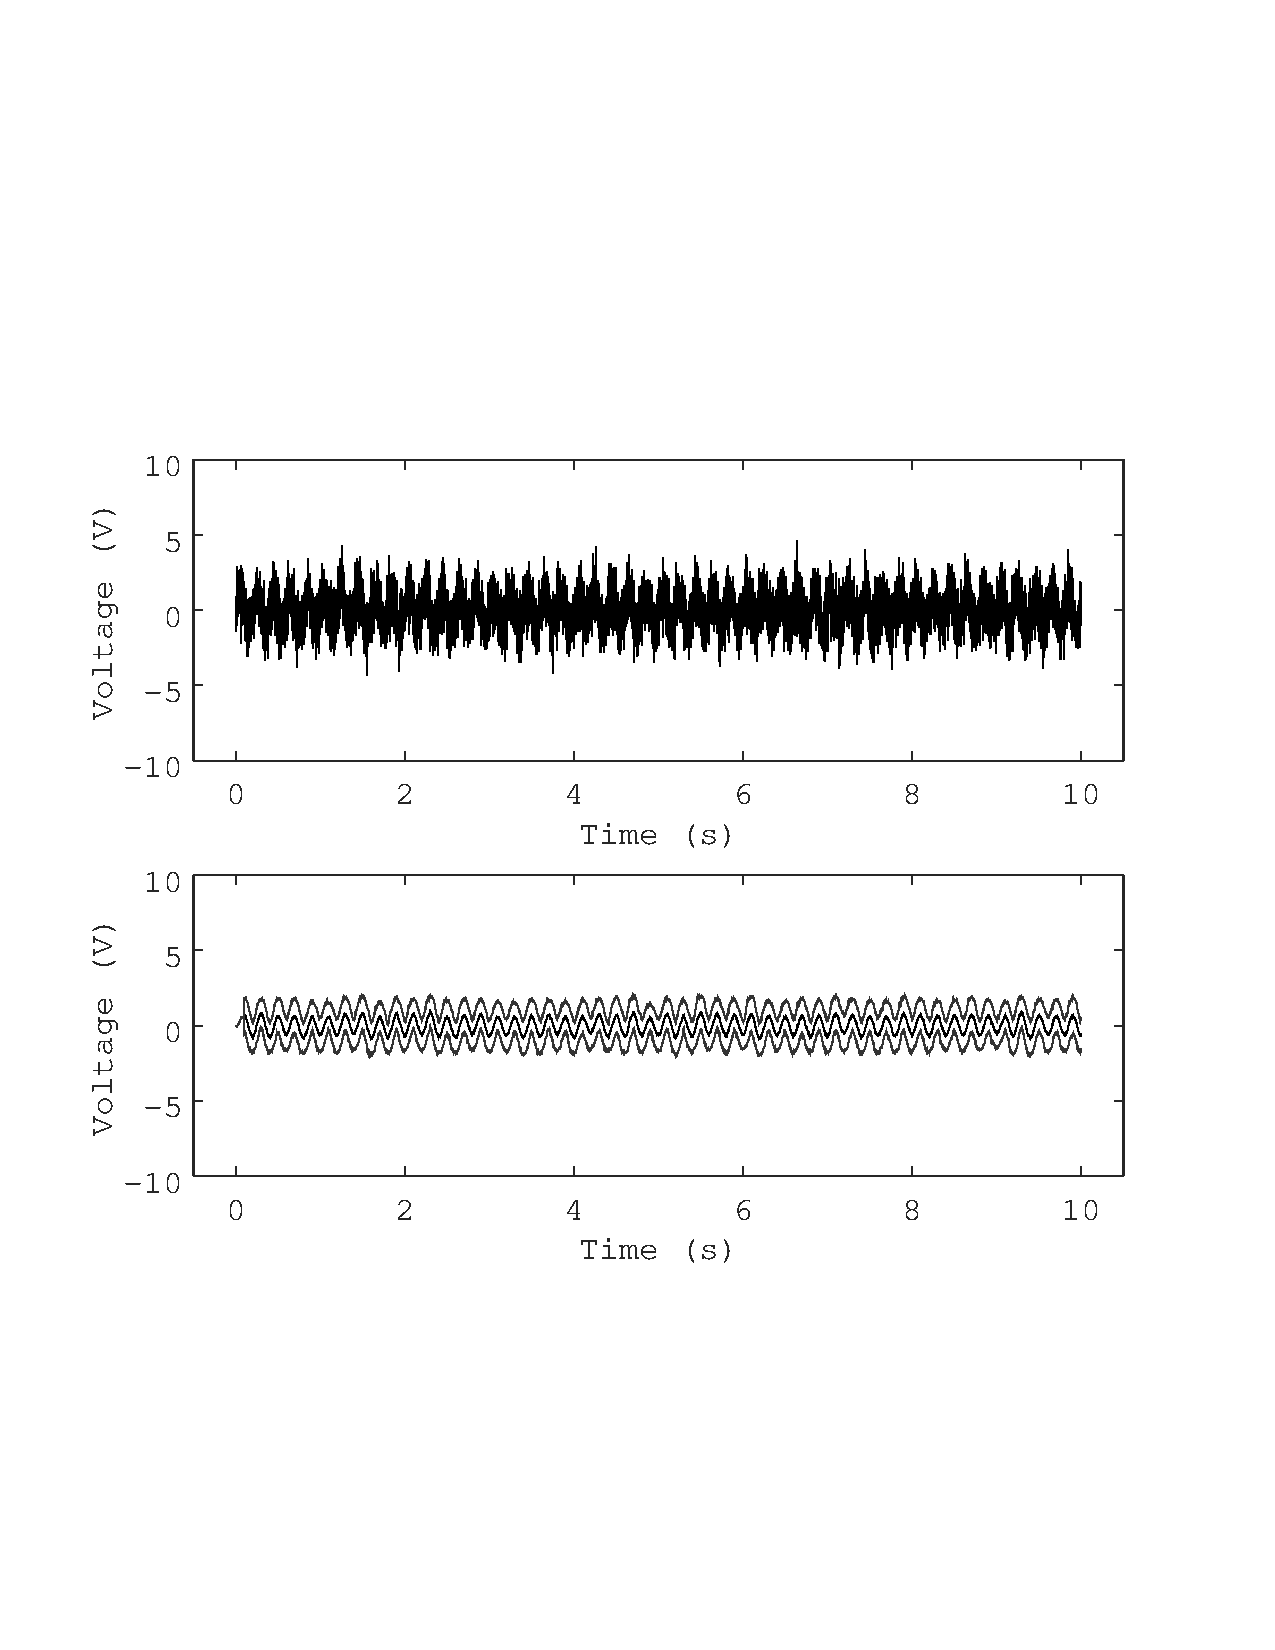
\includegraphics[width=0.5\textwidth,trim=0cm 6cm 0cm 6cm,clip=true]{figures/meanStdDev_plusCW.pdf}
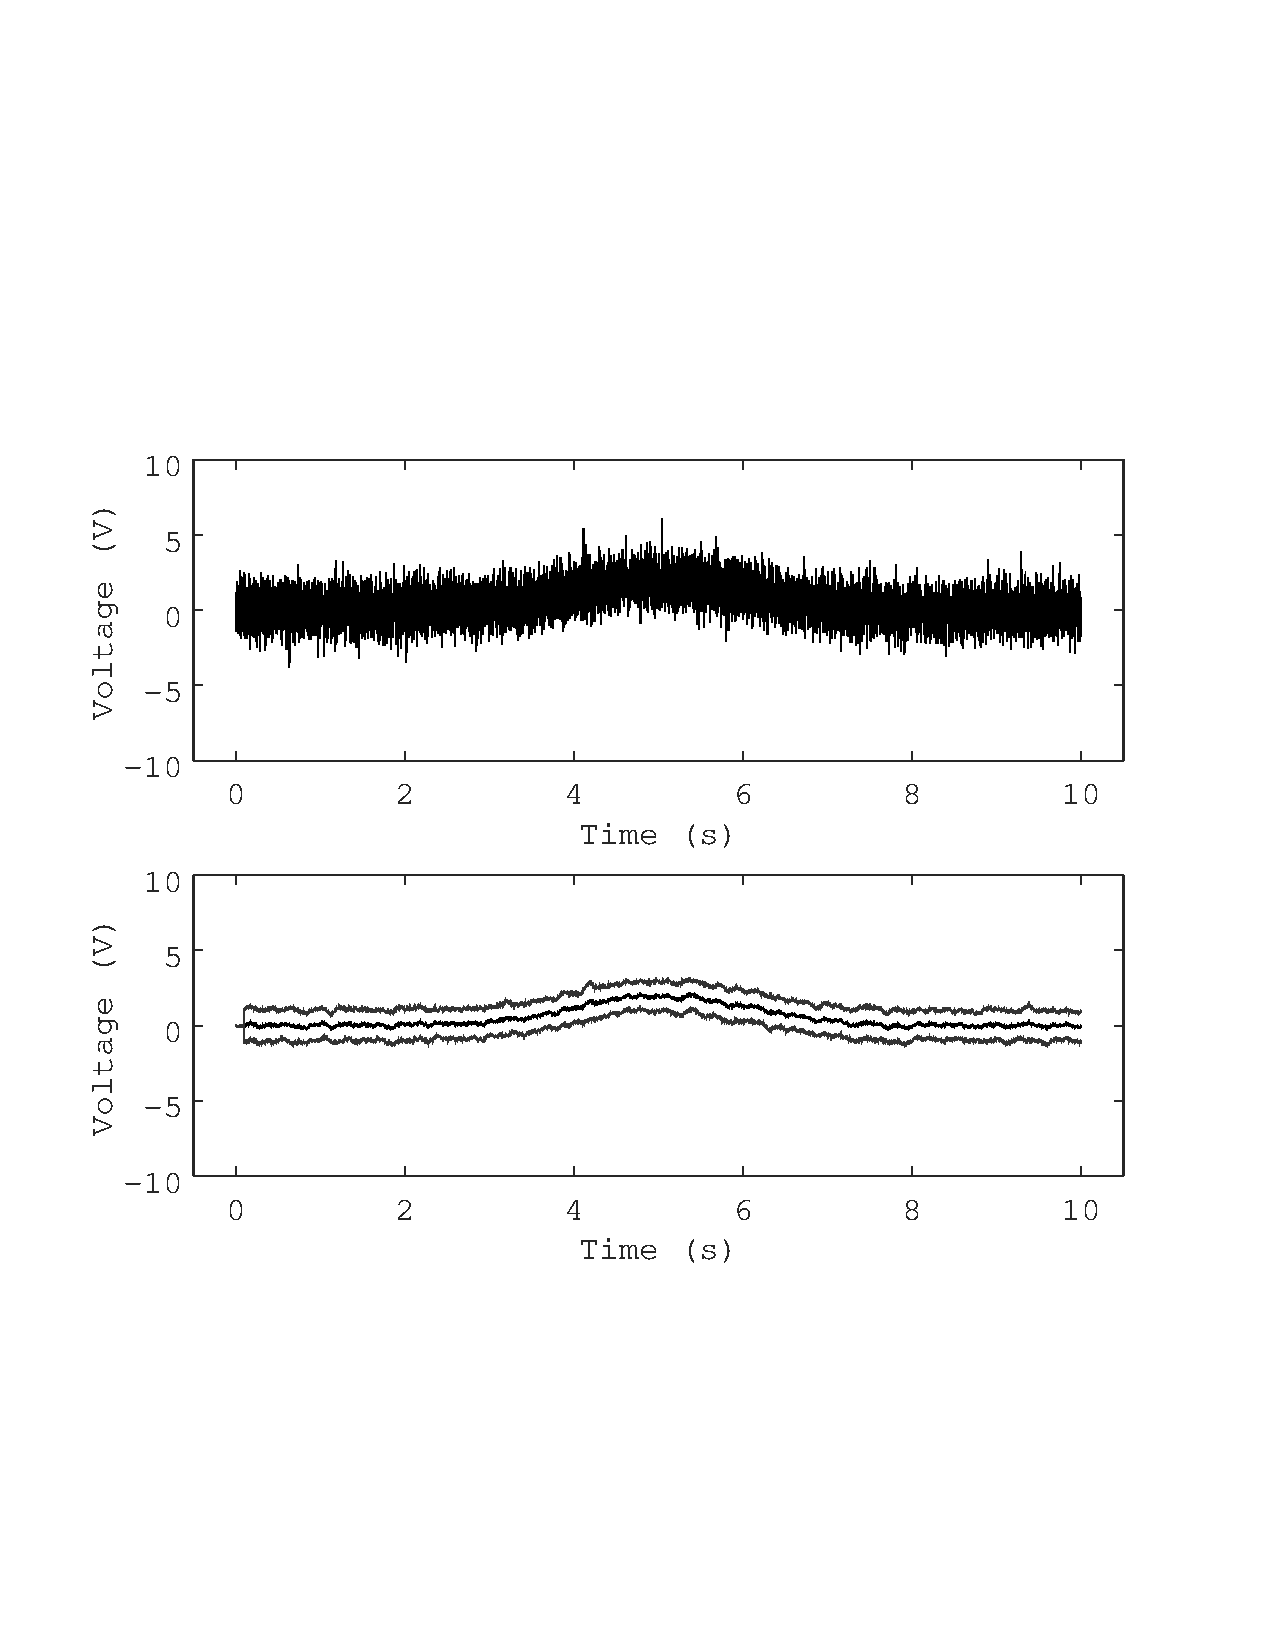
\includegraphics[width=0.5\textwidth,trim=0cm 6cm 0cm 6cm,clip=true]{figures/meanStdDev_plusGaussian.pdf}
\caption{\label{fig:dropin} (Left) A CW signal in the presence of normally distributed noise. (Right) A Gaussian pulse in the presence of normally distributed noise.}
\end{figure}
\end{frame}

\begin{frame}[fragile]{Statistics and Probability: Other Useful Distributions}
\small
Octave has many pre-programmed distributions.  Although system noise is usually normally distributed, it's good to know these:
\url{https://octave.org/doc/v4.2.0/Distributions.html} \\ \vspace{0.5cm}
Useful video on inverse transform sampling: \url{https://www.youtube.com/watch?v=rnBbYsysPaU&t=373s}
\end{frame}

\section{Supplement: Damped driven harmonic oscillator}

\begin{frame}{Supplement: Damped driven harmonic oscillator}
Let the defining equation for the signal $x(t)$ be
\begin{equation}
x'' + bx' + cx = A\cos(\omega_0 t)
\end{equation}
Take the Fourier transform of both sides:
\begin{equation}
\left((j\omega)^2 + j\omega b + c\right)X(\omega) = A \int_{-\infty}^{\infty} \cos(\omega_0 t) \exp(-j\omega t) dt
\end{equation}
The right-hand side is a pair of delta-functions:
\begin{equation}
F\lbrace \cos(\omega_0 t) \rbrace = \frac{1}{2}\left(\delta(\omega-\omega_0) + \delta(\omega+\omega_0)\right)
\end{equation}
\end{frame}

\begin{frame}{Supplement: Damped driven harmonic oscillator}
\small
Solving for $X(\omega)$ gives
\begin{equation}
X(\omega) = -\frac{A}{2}\frac{\delta(\omega-\omega_0) + \delta(\omega+\omega_0)}{\omega^2 + j\omega b + c}
\end{equation}
Taking the inverse Fourier transform gives
\begin{equation}
x(t) = -\frac{A}{4\pi}\left(\frac{\exp(-j\omega_0 t)}{\omega_0^2 + j\omega_0 b + c}+\frac{\exp(j\omega_0 t)}{\omega_0^2 + j\omega_0 b + c}\right)
\end{equation}
Let $k^2 = \omega_0^2-c$.  (Finish on board). Are there any special conditions you see (resonance, total damping)?  Can we plot this in Octave for varying damping and $c$ parameters?

\end{frame}

\section{Noise: Digitization and Sampling, theory and examples}

\begin{frame}[fragile]{Noise: Digitization and Sampling}
\begin{figure}
\centering
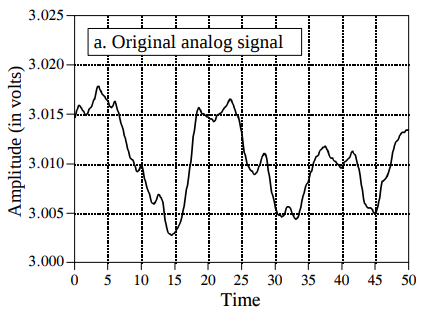
\includegraphics[width=0.6\textwidth]{figures/adc_dac1.png}
\caption{\label{fig:adc1} An example of analogue data from chapter 2 of the text.  Both the dependent and independent axes are continuous.}
\end{figure}
\end{frame}

\begin{frame}[fragile]{Noise: Digitization and Sampling}
\begin{figure}
\centering
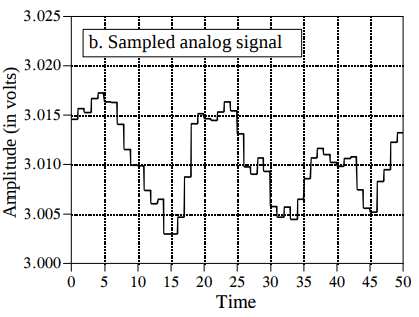
\includegraphics[width=0.6\textwidth]{figures/adc_dac2.png}
\caption{\label{fig:adc2} The same signal from Fig. \ref{fig:adc1}, except a \textit{sample-and-hold} action has been applied to the independent variable.}
\end{figure}
\end{frame}

\begin{frame}[fragile]{Noise: Digitization and Sampling}
\begin{figure}
\centering
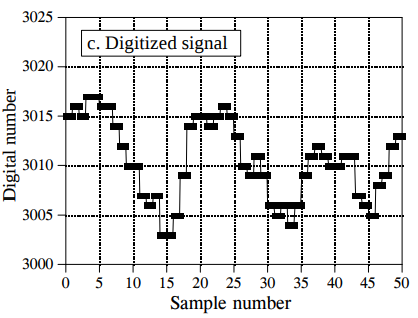
\includegraphics[width=0.6\textwidth]{figures/adc_dac3.png}
\caption{\label{fig:adc3} The same signal from Fig. \ref{fig:adc2}, except a \textit{digitization} action has been applied to the dependent variable.}
\end{figure}
\end{frame}

\begin{frame}[fragile]{Noise: Digitization and Sampling}
\begin{figure}
\centering
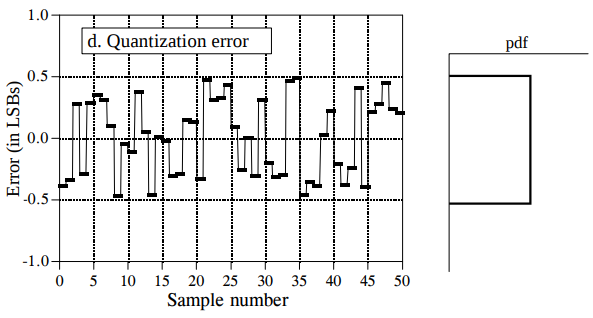
\includegraphics[width=0.6\textwidth]{figures/adc_dac4.png}
\caption{\label{fig:adc4} The error incurred by the \textit{digitization} action from Fig. \ref{fig:adc3}.  The y-axis is expressed in units of LSB (least significant bit - more in a second). Turns out we know the $\sigma$ of this error: $LSB/sqrt{12}$.}
\end{figure}
\end{frame}

\begin{frame}[fragile]{Noise: Digitization and Sampling}
A model for a particular value in Fig. \ref{fig:adc2}, the sample-and-hold action\footnote{Technically, this is the 0$^{th}$-order hold, and there are other (much) less common choices.} is
\begin{equation}
s_n(t) = f(n\Delta t) square(t-n\Delta t)
\end{equation}
where $f(n\Delta t)$ is the function or data value, and 
\begin{equation}
square(t) = 1, ~~~ |t| \leq T/2
\end{equation}
The entire $N$-sample data-set or signal is
\begin{equation}
s(t) = \sum_{n=0}^{N-1} f(n\Delta t) square(t-n\Delta t)
\end{equation}
\end{frame}

\begin{frame}[fragile]{Noise: Digitization and Sampling}
\begin{tcolorbox}[colback=white,colframe=red!40!blue,title=Sample/Hold Signal Model]
\alert{
\begin{equation}
s(t) = \sum_{n=0}^{N-1} f(n\Delta t) square(t-n\Delta t)
\end{equation}
}
\end{tcolorbox}
Several important questions:
\begin{enumerate}
\item What is $S(\omega)$?
\item What are the important relationships between $\Delta t$, $N$, and the frequencies present in the data?
\item How precisely does $s(t)$ represent the data?
\end{enumerate}
\end{frame}

\begin{frame}{Noise: Digitization and Sampling}
\small
The Fourier transform of $s(t)$ may be obtained using a combination of properties of the Fourier transform, plus the result obtained for $F\lbrace square(t) \rbrace$.  Let $x = \omega \Delta t/2$.  The result is (observe on board):
\begin{equation}
S(\omega) = sync(x) \sum_{n=0}^{N-1} f(n\Delta t) \exp(-j\omega n\Delta t) \Delta t \label{eq:awesome}
\end{equation}
The factor at right is a discrete version of the Fourier Transform.  Let the DFT represent the discrete Fourier transform on the right.  Equation \ref{eq:awesome} may be written
\begin{equation}
S(\omega) = DFT\lbrace f(t) \rbrace sync(x) 
\end{equation}
\alert{The spectrum of a sampled signal is the \textbf{convolution} of the discrete Fourier transform of the signal and the sync function with a period of the time between samples.}
\end{frame}

\begin{frame}{Noise: Digitization and Sampling}
The convolution of two functions $f(t)$ and $g(t)$ is 
\begin{equation}
(f \circ g) (t) = \int_{-\infty}^{\infty} f(\tau) g(t-\tau) d\tau
\end{equation}
\textbf{Convolution theorem}:  The Fourier transform of the convolution of two functions $f \circ g$ is
\begin{equation}
F\lbrace f \circ g\rbrace = F(\omega) G(\omega)
\end{equation}
\end{frame}

\begin{frame}{Noise: Digitization and Sampling}
The DFT can contain only have a finite number of frequencies, since it is discrete.  What are the limits of this?
\begin{figure}
\centering
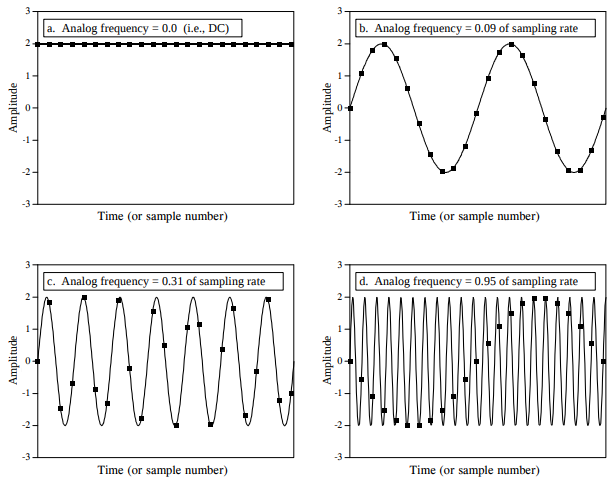
\includegraphics[width=0.6\textwidth]{figures/sampling.png}
\caption{\label{fig:sampling} Various degrees of sampling.}
\end{figure}
\end{frame}

\begin{frame}{Noise: Digitization and Sampling}
Notice that the sync function has a zero, which occurs at $x = \pi$, for some frequency $f_s$.  This implies that 
\begin{align}
\pi &= \frac{\omega \Delta t}{2} \\
\pi &= \frac{2\pi f_s \Delta t}{2} \\
f_s &= \frac{1}{\Delta t}
\end{align}
The frequency $f_s$ is known as the \textit{sampling frequency.}
\end{frame}

\begin{frame}{Noise: Digitization and Sampling}
We have finally arrived at the \textit{sampling theorem:}
\begin{tcolorbox}[colback=white,colframe=red!40!blue,title=Sampling Theorem]
\alert{A signal containing frequencies less than or equal to $f_{crit} = f_s/2$ can be perfectly reconstructed.}
\end{tcolorbox}
Let's go back and think about Fig. \ref{fig:sampling}.
\end{frame}

\begin{frame}{Noise: Digitization and Sampling}
The DFT can contain only have a finite number of frequencies, since it is discrete.  What are the limits of this?
\begin{figure}
\centering
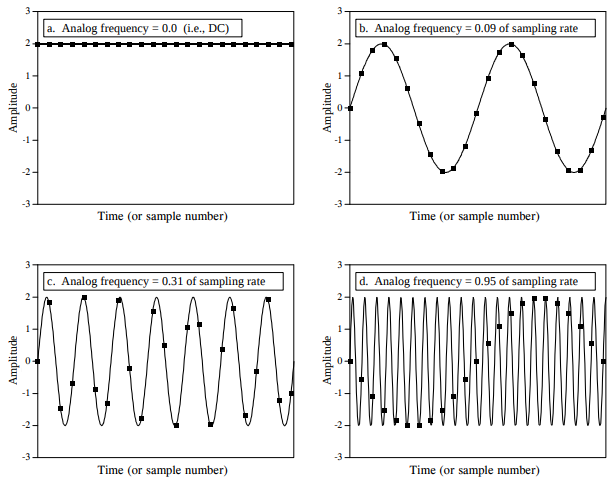
\includegraphics[width=0.6\textwidth]{figures/sampling.png}
\caption{\label{fig:sampling2} What if the sine wave had a frequency of $f_{c}$?. (Professor draw on board).}
\end{figure}
\end{frame}

\begin{frame}{Noise: Digitization and Sampling}
Equation \ref{eq:awesome} contained a form of the DFT.  Let $h(k\Delta t) = h_k$, with $f_s = 1/\Delta t$ and $N$ time samples. The discrete Fourier transform is defined as
\begin{equation}
H_n \approx \Delta t \sum_{k=0}^{N-1} h_k \exp\left( -2\pi j k \frac{n}{N} \right) \label{eq:fft1}
\end{equation}
The integral is approximated at frequencies $f_n = \frac{n}{N\Delta t}$. The inverse DFT is
\begin{equation}
h_k \approx \frac{\Delta f}{N}\sum_{n=0}^{N-1} H_n \exp\left( 2\pi j k \frac{n}{N} \right) \label{eq:fft2}
\end{equation}
What is $\Delta f$? There are $N/2$ \textit{independent frequencies} for real data, so $\Delta f = f_c/(N/2) = T^{-1}$.
\end{frame}

\begin{frame}{Noise: Digitization and Sampling}
\begin{figure}
\centering
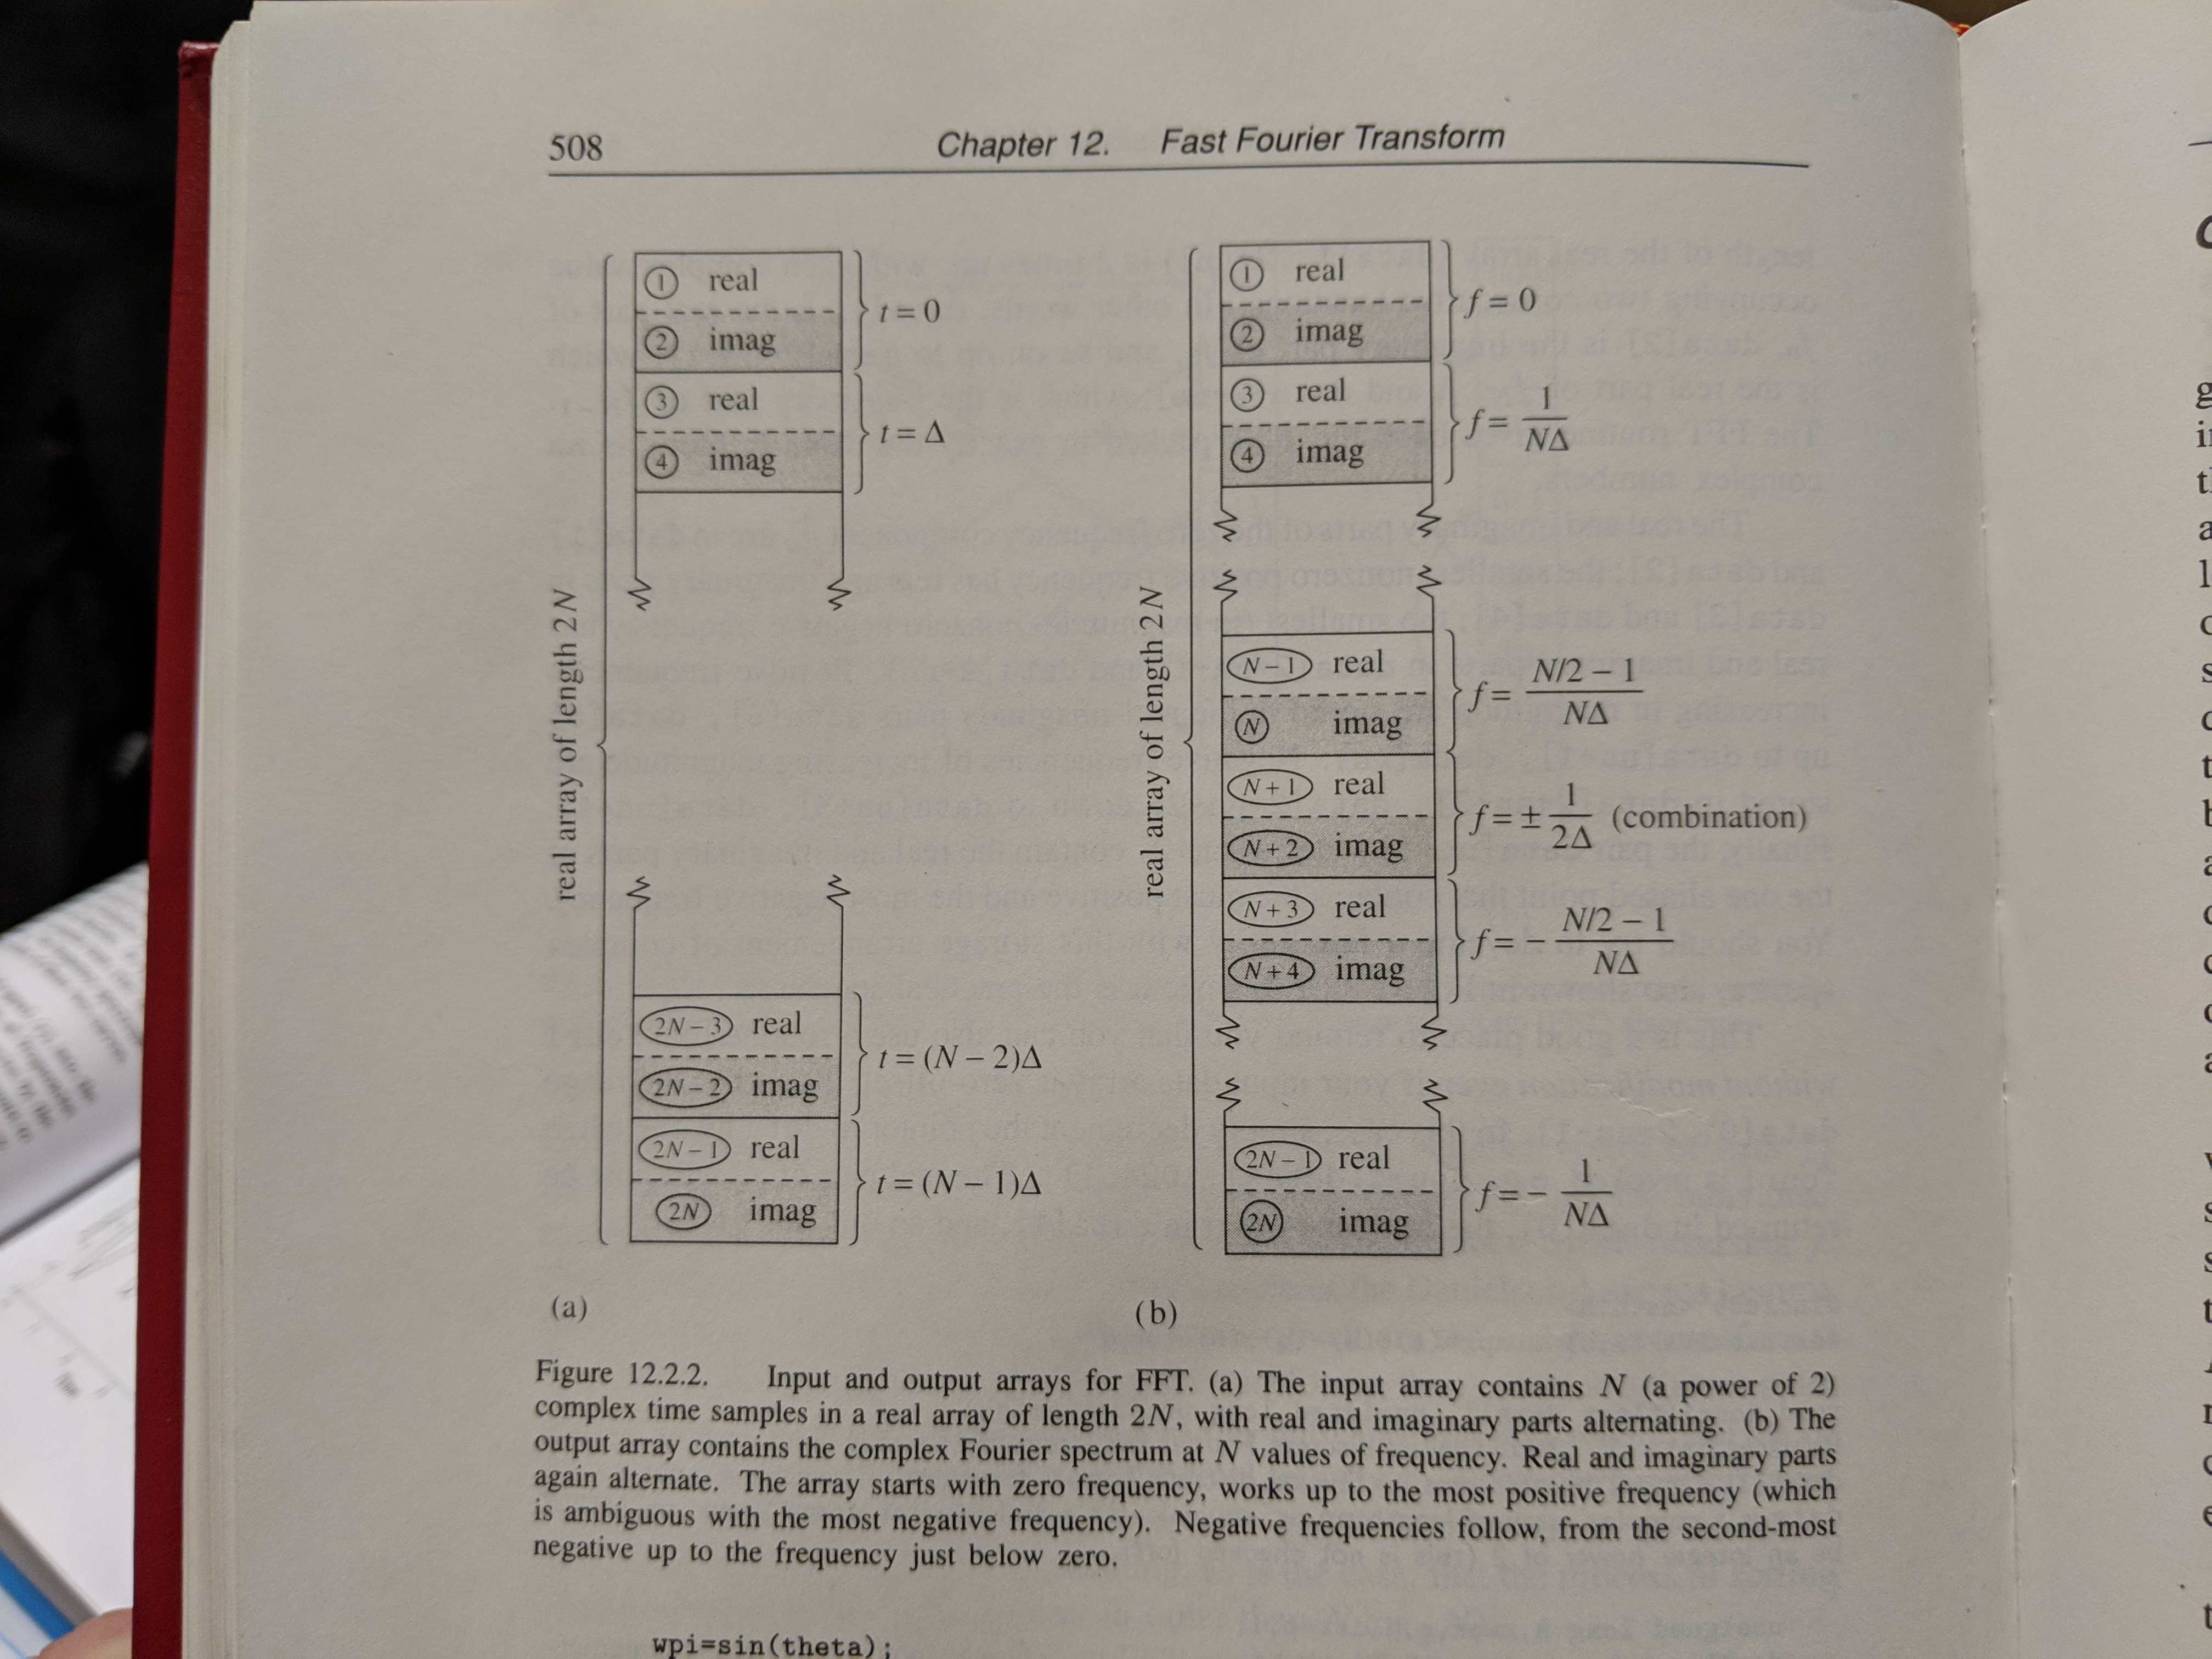
\includegraphics[width=0.75\textwidth,trim=21cm 25cm 18cm 12cm,clip=true]{figures/fft.jpg}
\caption{\label{fig:fft3} The FFT must conserve degrees of freedom.  The data are organized to optimize speed and efficiency.  (Left) Time samples. (Right) Frequency samples.}
\end{figure}
\end{frame}

\begin{frame}{Noise: Digitization and Sampling}
\small
Therefore in some implementations (\textbf{not} including octave) transforming forward and then backward incurs a factor of $N$. \\ \vspace{0.5cm}
Looking at Fig. \ref{fig:fft3}, let's do a few things:
\begin{enumerate}
\item Convince ourselves that $\Delta f = 1/T$.
\item Convince ourselves that degrees of freedom are conserved.
\item Convince ourselves that the data $\pm 1/2\Delta t$ should be the same.
\item Ensure we understand the order of the negative frequencies.
\end{enumerate}
Parseval's theorem works like this for the discrete quantities:
\begin{equation}
\sum_{k=0}^{N-1} |h_k|^2 = \frac{1}{N}\sum_{n=0}^{N-1} |H_n|^2
\end{equation}
\end{frame}

\section{Noise: Digitization and Sampling, Octave coding example}

\begin{frame}{Noise: Digitization and Sampling}
\small
How do we determine if data has been \textit{properly sampled} or \textit{properly sampled?} \textbf{Aliasing}.\footnote{This is apart from the trivial case when we know $f_s$ and $f_{max}$.} On Moodle, obtain the Aliasing.m script.
\begin{enumerate}
\item Activity: run for the first time, and take a few moments to understand the output. What are the units of the axes? What is the lower panel showing? 
\item Add noise by boosting the standard deviation of the pdf of the noise distribution by increasing the parameter \textbf{noise\_sigma}.
\item What happens to the amplitude when you increase the number of modes in the Fourier series?
\item Push the Fourier modes way above the sampling rate.  What happens to the amplitude?\footnote{Do you see the Gibb's phenomenon disappear?  Why?} \textit{Probably best to minimize noise.}
\end{enumerate}
\end{frame}

\begin{frame}{Noise: Digitization and Sampling}
\small
\textbf{Aliasing.} Building off of the Aliasing.m script, do the following:
\begin{enumerate}
\item \textit{Filter the data} according to the transfer function of the single-pole low-pass filter.
\item Use this technique to get rid of any aliasing, and explore the effect on the Fourier modes and noise.
\item Limit the Fourier series to $\approx 25$ terms, and use $f_0 \approx 1$ Hz.  Plot the signal while varying $f_{s}$.  What do you notice?
\end{enumerate}
Looks like adding noise in frequency-space where there is no signal just distorts the signal.  Does this make sense?
\end{frame}

\begin{frame}{Noise: Digitization and Sampling}
Now we return to the problem of precision due to \textit{digitization} in the \textit{dependent variable}, as opposed to \textit{sampling} in the independent variable. \\ \vspace{0.5cm}
Recall how the \textbf{\alert{standard deviation}} in the digitized dependent variable is $LSB/\sqrt{12}$.  Let's begin calling the least-significant bit (LSB) the quantum (Q).  Now imagine we are digitizing analog sinusoids between $-V/2$ and $V/2$ with $N$ quanta.  The standard deviation of data distributed like a sinusoid is $V/(2\sqrt{2})$.  Taking the ratio of the two standard deviations will give us the signal to noise ratio.
\end{frame}

\begin{frame}{Noise: Digitization and Sampling}
\small
Written in equation form, these ideas translate as follows:
\begin{align}
\sigma_{S} &= \frac{V}{2\sqrt{2}} = \frac{2^N Q}{2\sqrt{2}} \\
\sigma_{Q} &= \frac{Q}{\sqrt{12}} \\
\frac{\sigma_S}{\sigma_Q} &= \frac{\frac{2^N Q}{2\sqrt{2}}}{\frac{Q}{\sqrt{12}}} \\
\frac{\sigma_S}{\sigma_Q} &= \frac{2^N \sqrt{12}}{2\sqrt{2}} \label{eq:SNR1} \\
\end{align}
Often SNR is quoted in decibels.  The formula for decibel is 
\begin{equation}
P_{dB} = 10\log(P_2/P_1)
\end{equation}
Since $P \propto V^2$, 
\begin{equation}
P_{dB} = 20\log(V_2/V_1)
\end{equation}
\end{frame}

\begin{frame}{Noise: Digitization and Sampling}
\small
Applying the definition of decibel to Eq. \ref{eq:SNR1}:
\begin{align}
SNR_{dB} &= 20\log\left(\frac{2^N \sqrt{12}}{2\sqrt{2}} \right) \\
SNR_{dB} &= 20 N \log(2) + 20\log(\sqrt{6}/2) \\
SNR_{dB} &= 6.02 N + 1.76
\end{align}
Example: in the presence of \textit{just} quantization noise, if we digitize with 8 bits, we expect an SNR $\approx 50$ dB.  What if we drop to 4 bits? Answer: $\approx 26$ dB.  What if there is \textit{analogue} noise in addition to the \textit{quantization} noise?  Suppose it has standard deviation of $\sigma_N$.
\begin{equation}
\frac{\sigma_S}{\sigma_Q+\sigma_N} = \frac{\frac{2^N Q}{2\sqrt{2}}}{\frac{Q}{\sqrt{12}} + \sigma_N}
\end{equation}
\end{frame}

\begin{frame}{Noise: Digitization and Sampling}
\small
\begin{equation}
SNR_{dB} = 6.02 N + 1.76 - 20\log\left( 1 + \sqrt{12} \frac{\sigma_N}{Q}\right)
\end{equation}
Recalling that $\sigma_Q = Q/\sqrt{12}$, we have
\begin{equation}
SNR_{dB} = 6.02 N + 1.76 - 20\log\left( 1 + \frac{\sigma_N}{\sigma_Q}\right)
\end{equation}
\textbf{Example:} suppose we have $\sigma_N = 20$ mV, and we have $N=8$ bits over a 2.56 V range.  This means $\sigma_Q = 2.56/256/\sqrt{12} = 1/(100\sqrt{12}) \approx 2.89$ mV.  Thus, $\sigma_N/\sigma_Q = 20/2.89 \approx 6.92$.  The final answer is then $SNR_{dB} = 32$.  This is the maximum achievable SNR (in decibels) in this system.\footnote{More realistically, the noises add in quadrature, but in practice the system is designed so that $\sigma_N$ dominates over $\sigma_Q$.}
\end{frame}

\begin{frame}{Noise: Digitization and Sampling}
\small
What are the maximum SNR values in dB acheivable on the following systems?
\begin{enumerate}
\item 16 bits, 6.55V, with $50$ mV of analogue noise.
\item 12 bits, 4.096V, with $50$ mV of analogue noise.
\item 12 bits, 4.096V, with $5$ mV of analogue noise.
\end{enumerate}
\end{frame}

\begin{frame}{Noise: Digitization and Sampling}
\begin{figure}
\centering
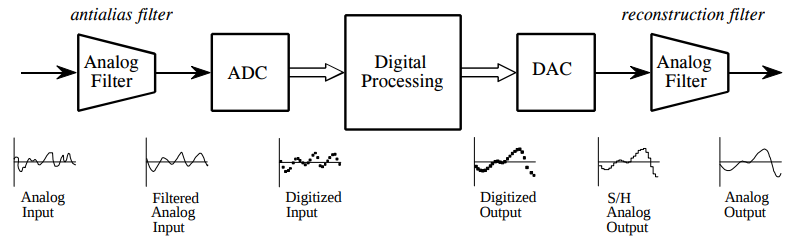
\includegraphics[width=0.75\textwidth]{figures/recon.png}
\caption{\label{fig:fulladc} The complete (basic) system for sampling and digitization, reconstruction.}
\end{figure}
\end{frame}

\begin{frame}{Noise: Digitization and Sampling}
\small
We already know what the reconstruction filter should be: the inverse of the sync function encountered in the derivation of the sampling theorem ideas. \\ \vspace{0.5cm}
What type of anti-aliasing filter should be chosen?  Chapter 3 of the text covers three:
\begin{enumerate}
\item Butterworth
\item Bessel
\item Chebyshev
\end{enumerate}
But this begs the question.  How do filters work in general?  Besides the single-pole examples we've already seen, what other types are there? \\
We have now reached \textbf{Unit 2!}
\end{frame}

\section{Conclusion}

\begin{frame}{Unit 1.3 Outline}
Previous lectures covered:
\begin{itemize}
\item Complex numbers 2: The Fourier series and Fourier transform (continuous and discrete)
\item \textit{Time-permitting}: The Laplace transform (continuous and discrete)
\end{itemize}
This lecture will cover: (Reading: \textbf{Chapter 2})
\begin{itemize}
\item \alert{Statistics and probability: the normal distribution and other useful distributions}
\item \alert{Noise: digitization and sampling}
\item \alert{Noise: Spectral properties of noise, ADC and DAC}
\end{itemize}
\end{frame}

\end{document}
